\documentclass[11pt, a4paper, subeqn]{article}
\usepackage[english]{babel}
\usepackage{graphicx}
\usepackage{comment}
\usepackage{amsmath}
\usepackage{amssymb}
\usepackage{psfrag}
\usepackage{bm}
%\usepackage[a4paper, width=15.5cm, height=24.7cm]{geometry}

% $Header$
% Copyright (C) 1996-2023 Pierangelo Masarati <pierangelo.masarati@polimi.it>
% Dipartimento di Ingegneria Aerospaziale, Politecnico di Milano
%
% Parentesi: tonde, quadre, curly, dritte, doppie e angolari.
\newcommand{\plbr}[1]{ \left( #1 \right) }
\newcommand{\sqbr}[1]{ \left[ #1 \right] }
\newcommand{\cubr}[1]{ \left\{ #1 \right\} }
\newcommand{\shbr}[1]{ \left| #1 \right| }
\newcommand{\nrbr}[1]{ \left\| #1 \right\| }
\newcommand{\anbr}[1]{ \langle #1 \rangle }

% Parentesi solo a sinistra: tonde, quadre, curly, dritte, doppie e angolari.
\newcommand{\lplbr}[1]{ \left( #1 \right. }
\newcommand{\lsqbr}[1]{ \left[ #1 \right. }
\newcommand{\lcubr}[1]{ \left\{ #1 \right. }
\newcommand{\lshbr}[1]{ \left| #1 \right. }
\newcommand{\lnrbr}[1]{ \left\| #1 \right. }
\newcommand{\lanbr}[1]{ \langle #1 \right. }

% Parentesi solo a destra: tonde, quadre, curly, dritte,doppie e angolari.
\newcommand{\rplbr}[1]{ \left. #1 \right) }
\newcommand{\rsqbr}[1]{ \left. #1 \right] }
\newcommand{\rcubr}[1]{ \left. #1 \right\} }
\newcommand{\rshbr}[1]{ \left. #1 \right| }
\newcommand{\rnrbr}[1]{ \left. #1 \right\| }
\newcommand{\ranbr}[1]{ \left. #1 \rangle }

% Vettori verticali:
\newcommand{\vvect}[2]{ \begin{array}{ #1 } #2 \end{array} }
\newcommand{\cvvect}[1]{ \begin{array}{c} #1 \end{array} }
\newcommand{\lvvect}[1]{ \begin{array}{l} #1 \end{array} }
\newcommand{\rvvect}[1]{ \begin{array}{r} #1 \end{array} }

% Vettori orizzontali:
\newcommand{\hvect}[2]{ \begin{array}{ #1 } #2 \end{array} }

% Matrici:
\newcommand{\matr}[2]{ \begin{array}{ #1 } #2 \end{array} }

% Integrali: uso \intg{inf}{sup}{arg}{dvar}
\newcommand{\intg}[4]{ \int_{#1}^{#2} {#3} \ {#4} }

% Limite: uso \limt{var}{lim}{arg}
\newcommand{\limt}[3]{ \lim_{{#1} \rightarrow {#2}} {#3}}

% LogLike functions
\newcommand{\llk}[1]{\ensuremath{\mathrm{#1}}}

\newcommand{\diag}[0]{\llk{diag}}
\newcommand{\tr}[0]{\llk{tr}}
\newcommand{\sym}[0]{\llk{sym}}
\newcommand{\skw}[0]{\llk{skw}}

\newcommand{\step}[0]{\llk{step}}
\newcommand{\imp}[0]{\llk{imp}}

\newcommand{\grad}[0]{\llk{grad}}
\newcommand{\divr}[0]{\llk{div}}
\newcommand{\rot}[0]{\llk{rot}}

% In italiano ...
\newcommand{\sca}[0]{\llk{sca}}

% first, second, etc
\newcommand{\first}[0]{1\ensuremath{^{\mathrm{st}}}}    % 1^st
\newcommand{\second}[0]{2\ensuremath{^{\mathrm{nd}}}}   % 2^nd
\newcommand{\third}[0]{3\ensuremath{^{\mathrm{rd}}}}    % 3^rd
\newcommand{\rth}[0]{\ensuremath{^{\mathrm{th}}}}       %  ^th

\newcommand{\degr}[0]{\ensuremath{^{\mathrm{o}}}}

% esponenziale
\providecommand{\e}[1]{\llk{e}^{#1}}

\newcommand{\T}[1]{\bm{\mathbf #1}}
\newcommand{\TT}[1]{\bm{\mathbf #1}}

\begin{document}

\title{Analysis of DETC2007-35511 Model using MBDyn}

\author{Pierangelo Masarati \\
Politecnico di Milano, Dipartimento di Ingegneria Aerospaziale \\
masarati@aero.polimi.it}

% \date{\today}
\date{August 21, 2009}

\maketitle

\section*{Introduction}
This document describes the modeling of the problem
discussed in \cite{MACLEAN-2007} using the free general-purpose
multibody software MBDyn \cite{MBDYN-WWW}.
The problem consists in a very slender beam, representative of a robot arm
for space applications, pinned at one end, and carrying a mass
at the other end.

The problem is originally formulated in analytical form as the free vibration
of a slender uniform beam.
Its boundary conditions consist in having zero transverse displacement
and bending moment at the pinned end, and zero bending moment at the free end.
The transverse shear force at the tip is represented by the inertia force
exerted by the lumped mass.

The original solution uses a modal approach.
The vibration modes of the problem are computed.
The resulting system is subjected to a given torque pattern applied
at the pinned end by an ideal DC motor.
The load pattern is illustrated in Figure~\ref{fig:torque-1}.

\begin{figure}
\centering
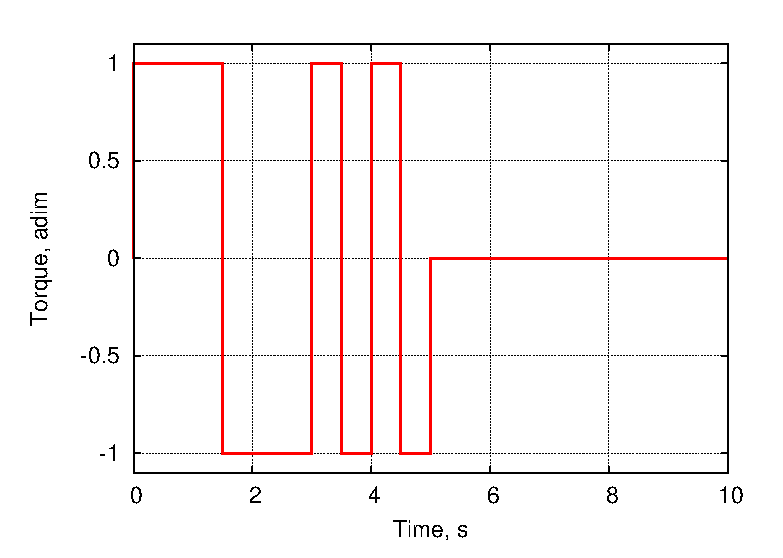
\includegraphics[width=.8\textwidth]{torque-1.eps}
\caption{Torque application pattern}
\label{fig:torque-1}
\end{figure}

Two models have been prepared:
\begin{enumerate}
\item a model that uses a similar approach, called `modal' in the results;
\item a model based on directly modeling the deformability of the slender
beam using the finite element method, with geometrically exact, nonlinear 
beam elements \cite{FV-AIAA}.
This model has been analyzed using increasingly refined meshes
(10 and 20 nodes).
\end{enumerate}

Data in SI units has been taken from \cite{MACLEAN-2007}.
As a first verification, Table~\ref{tab:modes} reports the results
of a modal analysis on the models used in the analysis,
compared to the results reported in \cite{MACLEAN-2007}.
All models show a pretty good agreement.
There is a discrepancy of 1.8\% on the first frequency that puzzles
a little bit, since the coefficients in matrices $M_{ee}$ and $K_{ee}$
have been computed according to the formulas provided in \cite{MACLEAN-2007}.


\begin{table}
\centering
\caption{Modal analysis results [rad/s]}
\label{tab:modes}
\begin{tabular}{lrrrr}
\hline
Mode & original & `modal' & \multicolumn{2}{c}{`beam'} \\
& & & 10 nodes & 20 nodes \\
\hline\hline
\#1	& 5.28	& 5.38	& 5.27	& 5.28 \\
\#2	& 20.9	& 20.9	& 20.7	& 20.8 \\
\#3	& 46.7	& 46.9	& 46.0	& 46.6 \\
\#4	& 83.4	& 83.6	& 80.8	& 82.4 \\
\hline
\end{tabular}
\end{table}

\section*{Modeling Issues}
Few issues surfaced.

\begin{enumerate}
\item Table~2 of \cite{MACLEAN-2007} reports four frequencies $\omega_i$ 
and four parameters $\mu_i$.
However, considering the relationship between $\omega_i$ and $\mu_i$,
given by Eq.~(23) in \cite{MACLEAN-2007} and reported below for clarity,
\begin{align}
	\omega_i
	&=
	\frac{\mu_i^2}{l^2} \sqrt{\frac{EI}{\rho}}
	,
\end{align}
the fourth value of $\omega_i$, 83.4 radian/s, is not consistent
with the fourth value of $\mu_i$, 15.71404495 m.
As a consequence, in the analysis 5 modes have been considered,
the first four with frequencies taken from Table~2 of \cite{MACLEAN-2007},
and the fifth computed from $\mu_i$ = 15.71404495, resulting in
$\omega_5$ = 129.7 radian/s.

\item The value of the torque shown in Figure~7 of \cite{MACLEAN-2007},
some 44 Nm, yields a motion that is about 10 times larger than the one
depicted in Figures~8 and 10 of \cite{MACLEAN-2007}.
Probably, some unit conversion error occurred, and the actual torque
applied in the analysis was lower.
By trial and error, a torque amplitude of 4.85 Nm appears to yield
comparable results.
\end{enumerate}

\section*{Numerical Results}
Figure~\ref{fig:tip-y} shows the transverse motion of the tip of the beam.
It is the equivalent of Figure~8 of \cite{MACLEAN-2007}.
Figure~\ref{fig:root-a} shows the rotation of the pinned end of the beam.
It is the equivalent of Figure~10 of \cite{MACLEAN-2007}.

\begin{figure}
\centering
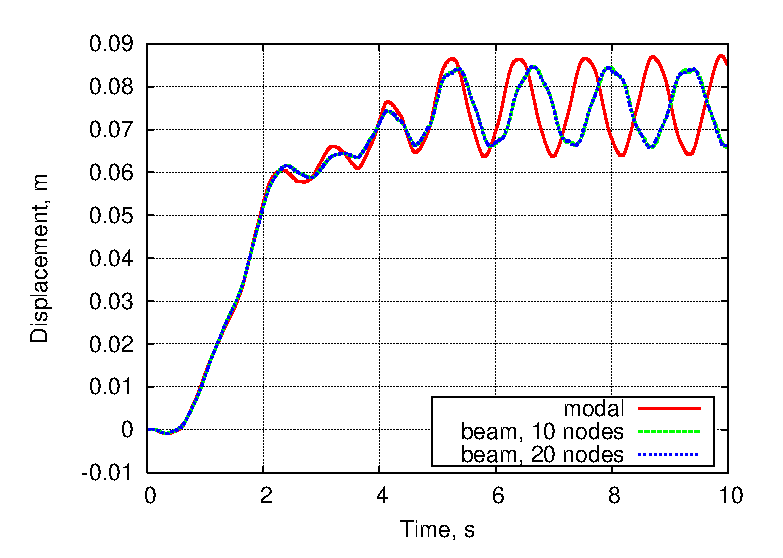
\includegraphics[width=.8\textwidth]{tip-y.eps}
\caption{Tip position}
\label{fig:tip-y}
\end{figure}

\begin{figure}
\centering
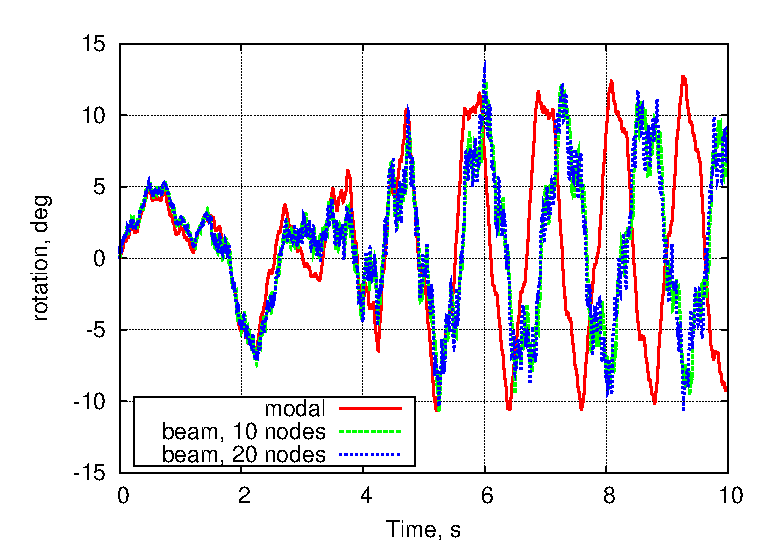
\includegraphics[width=.8\textwidth]{root-a.eps}
\caption{Root rotation}
\label{fig:root-a}
\end{figure}

The figure clearly shows that the `modal' model, based on a modal element,
provides results comparable to those in \cite{MACLEAN-2007}.
The models based on FEM modeling of the beam directly in the multibody
analysis yields somewhat different results.

The pattern is quite similar.  However, the essentially steady vibrations
at the first frequency of the system, ~0.85 Hz, appear with a slightly
reduced frequency, ~0.75 Hz.
This issue is not dictated by numerical problems: the integration time step
is 0.001 s, definitely enough for the accurate integration of dynamics
of the order of 1 Hz (0.01 s would suffice).

Since the beam is very slender, with a very large mass
($> 5$ times that of the beam) at the tip, its dynamics may nonlinearly depend
on the amplitude of the motion.
In fact, the critical buckling load for this configuration
(assuming it is instantaneously comparable to pinned-pinned),
is $N_\text{critical}=-EI(\pi/l)^2 = -87$ N.
The FEM analysis shows (Figure~\ref{fig:axial})
that the axial load in the beam oscillates in a pronounced manner,
with negative peaks well below this value.
This may heavily impact the dynamics of transverse vibrations,
as the transverse vibration frequency depends on the axial load
according to
\begin{align}
	\omega
	&=
	\plbr{\cfrac{\pi}{l}}^2 \sqrt{\frac{EJ}{\rho}}
		\sqrt{1 - \frac{N}{N_{\text{critical}}}}
	.
\end{align}

Another potential issue is that the modal model is based on a pinned
end assumption, so the mode shapes comply with a zero torque
boundary condition.
However, the input is represented by an imposed torque at the pinned end.
This may represent another source of potential error.

\begin{figure}
\centering
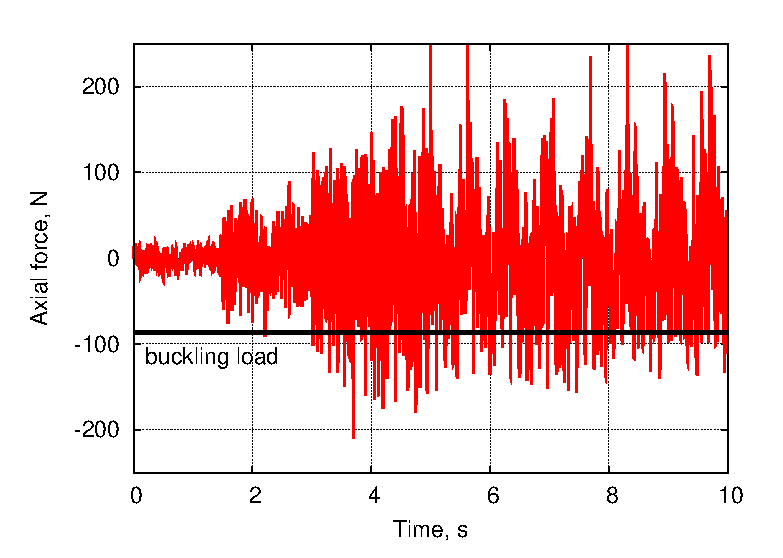
\includegraphics[width=.8\textwidth]{axial.eps}
\caption{Axial force in the beam}
\label{fig:axial}
\end{figure}


\bibliographystyle{unsrt}
\bibliography{mybib,DETC2007_35511}

\end{document}
